\documentclass[compress, aspectratio=169]{beamer}

\usefonttheme{professionalfonts}

\usepackage{fontspec}
\usepackage{polyglossia}
\setmainlanguage{german}

\usepackage{mathtools}
\usepackage[
  math-style=ISO,
  bold-style=ISO,
  nabla=upright,
  partial=upright,
]{unicode-math}

\usepackage[locale=DE, math-rm=\mathup]{siunitx}
\DeclareSIUnit{\year}{a}

\usepackage{graphicx}

\usepackage{tikz}
\usetikzlibrary{arrows}
\usetikzlibrary{arrows.meta}

\usepackage{pgfplots}
\usepgfplotslibrary{polar}
\pgfplotsset{compat=1.12}

\newcommand\fullscreenimage[1]{{%
  \usebackgroundtemplate{%
    \includegraphics[
      width=\paperwidth,
      height=\paperheight,
  ]{#1}}
  \begin{frame}[plain]%
  \end{frame}%
}}


\usepackage{xfrac}


\usetheme{vertex}

\newcommand\SIQ[2]{\ensuremath{#1\mathrel{/}\si{#2}}}
\newcommand\PI{\ensuremath{\mathup{π}}}
\newcommand\kb{\ensuremath{k_\mathup{B}}}
\newcommand\TB{\ensuremath{T_\mathup{B}}}


\author{Maximilian Nöthe}
\date[21.5.2015]{Seminar Radioastronomie, TU Dortmund, 21.5.2015}
\title{Das Wasserstoffspektrum}
\subtitle{in der Radioastronomie}

\begin{document}
\maketitle

\section{Linien-Emission}
\begin{frame}{Einstein-Koeffizienten}
  \begin{columns}[T, onlytextwidth]%
    \begin{column}{0.5\textwidth}%
      \begin{tikzpicture}[
  scale=0.75,
  level/.style={very thick},
  photon/.style={-{Stealth[length=2mm]}, color=red!70!black, thick, decorate, decoration={snake, pre length=0.5mm, post length=1mm,}},
  connect/.style={dashed, very thick},
  ]
  \draw[level] (0,  0) node [left] {$E_2$} -- +(8, 0);
  \draw[level] (0, -2) node [left] {$E_1$} -- +(8, 0);
  \draw[photon] (2, 0) -- +(0,-2) node [below] {\normalcolor Emission} node[midway,left] {$A_{21}$};
  \draw[photon] (4,-2) -- +(0, 2) node [above] {\normalcolor Absortion} node[midway,left] {$B_{12}\bar{U}$};
  \draw[photon] (6, 0) -- +(0,-2) node [below] {\normalcolor stim.\ Emission} node[midway, right] {$B_{21}\bar{U}$};
  \draw[photon] (5,-1) -- +(0.95, 0);
\end{tikzpicture}
%
    \end{column}%
    \begin{column}{0.45\textwidth}%
      mittlere Energiedichte:
      \begin{equation*}
        \bar{U} = \frac{4\PI}{c} \bar{I}
      \end{equation*}
      in statischem System:
      \begin{equation*}
        N_2 A_{21} + N_2 B_{21} \bar{U} = N_1 B_{12} \bar{U}
      \end{equation*}
    \end{column}%
  \end{columns}%
\end{frame}

\begin{frame}{Wichtige Kenngrößen}
  \begin{block}{Brightness Temperature $T_\mathup{B}$}
    \begin{align*}%
      \TB &= \frac{c²}{2 \kb} \frac{1}{ν²} I_ν & 
      \TB &= \frac{h ν}{k_\mathup{B}}
             \frac{1}{\ln\!\left(
                \frac{8\PI h ν³}{c³\bar{U}} + 1
             \right)} \\
      &\text{(allgemein)} &  &\text{(Linienemission)}
    \end{align*}%
  \begin{itemize}
    \item Rayleigh–Jeans-Temperatur für gegebene Intensität $I_ν$
    \item verbreitetes Helligkeitsmaß in der Radioastronomie
  \end{itemize}
  \end{block}%
\end{frame}

\begin{frame}{Die \SI{21}{\centi\meter}-Linie}
  \begin{columns}[c, onlytextwidth]%
    \begin{column}{0.6\textwidth}%
      \begin{tikzpicture}[
    level/.style={very thick},
  photon/.style={-{Stealth[length=2mm]}, thick, decorate, decoration={snake, pre length=1mm, post length=2mm,}}, connect/.style={dashed, very thick},
  ]
  \draw[level] (0, 0) -- (+1.5, 0) node at (0, 0) [above] {$1^2S_{\sfrac{1}{2}}$};
  \draw[connect] (1.5, 0) -- +(1.5,  1);
  \draw[connect] (1.5, 0) -- +(1.5, -1);
  \draw[level] (3,  1) -- +(1.5, 0);
  \draw[level] (3, -1) -- +(1.5, 0);

  \draw[red!70!black, ->, thick] (3.75, 1) -- +(0, -2)
    node[right, midway] {$\increment E = \SI{5.9e-6}{\electronvolt}$};
  \draw[red!70!black, photon] (3.75, 0) -- + (-3, -2)
  node[below, align=left] {$λ = \SI{21.11}{\centi\meter}$ \\ $f = \SI{1420.406}{\mega\hertz}$};
  \node[] at (5,  1) {$\uparrow \quad \uparrow$};
  \node[] at (5, -1) {$\uparrow \quad \downarrow$};
  \node[] at (5,  1.5) {$\mathup{p}\quad\mathup{e}$};
\end{tikzpicture}

    \end{column}%
    \begin{column}{0.4\textwidth}%
      \begin{itemize}
        \item Hyperfeinstruktur-Übergang in neutralem H
        \item stark unterdrückt:
          \begin{gather*}
            A_{21} = \SI{2.869}{\per\second} \\
            τ = \SI{1.1e7}{\year}
          \end{gather*}\vspace{-1.5\baselineskip}%
        \item Anregung durch Stöße im interstellarem Medium
      \end{itemize}
    \end{column}%
  \end{columns}%
\end{frame}

\begin{frame}{Geschichte}%
  \begin{columns}[c, onlytextwidth]%
    \column{0.15\textwidth}%
      \centering
      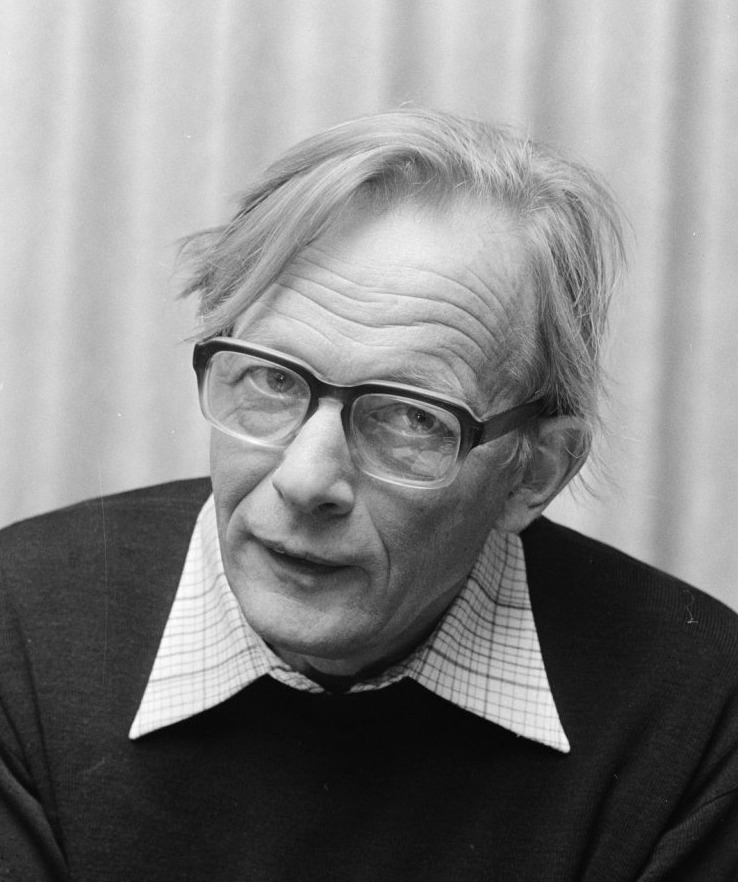
\includegraphics[width=\linewidth]{./images/Hendrik_vanDeHulst.jpg}
      \newline H. v.\,d. Hulst
    \column{0.8\textwidth}%
      \begin{description}[Hendrik van de Hulst]
        \item[Hendrik van de Hulst] Holländischer Astronom \& Mathematiker
        \item[1944] Vorhersage der \SI{21}{\centi\meter}-Linie
        \item[später] Mitarbeit bei der Kartographie der Milchstraße
      \end{description}
  \end{columns}%
  \vfill
  \begin{columns}[c, onlytextwidth]%
    \column{0.15\textwidth}%
      \centering
      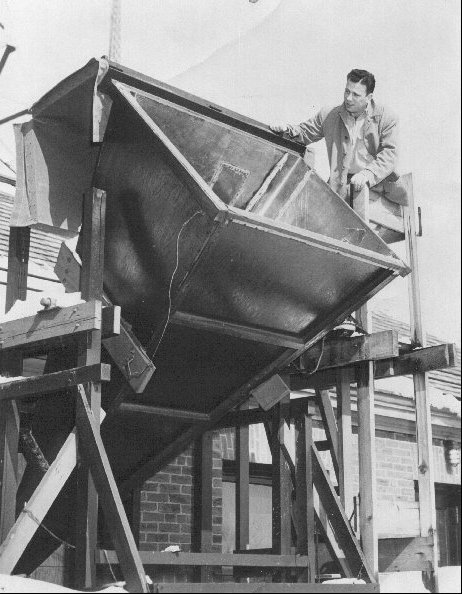
\includegraphics[width=\linewidth]{./images/ewenhorn.jpg}%
      \newline H.~Ewen
    \column{0.65\textwidth}%
      \begin{description}[1951]
        \item[1951] Entdeckung durch Edward Purcell \& Harold Ewen\\
                    an der Harvard University
      \end{description}
    \column{0.15\textwidth}%
      \centering
      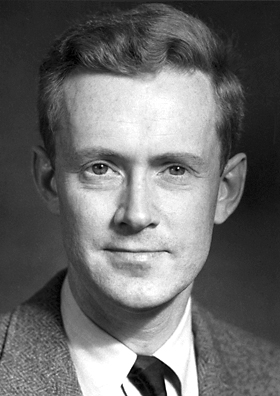
\includegraphics[width=\linewidth]{./images/Edward_Mills_Purcell.jpg}%
      \newline E.~Purcell
  \end{columns}%
\end{frame}

\begin{frame}{Die \SI{21}{\centi\meter}-Linie – Vermessung der Milchstraße}%
  \begin{columns}[c]%
    \begin{column}{0.5\textwidth}%
      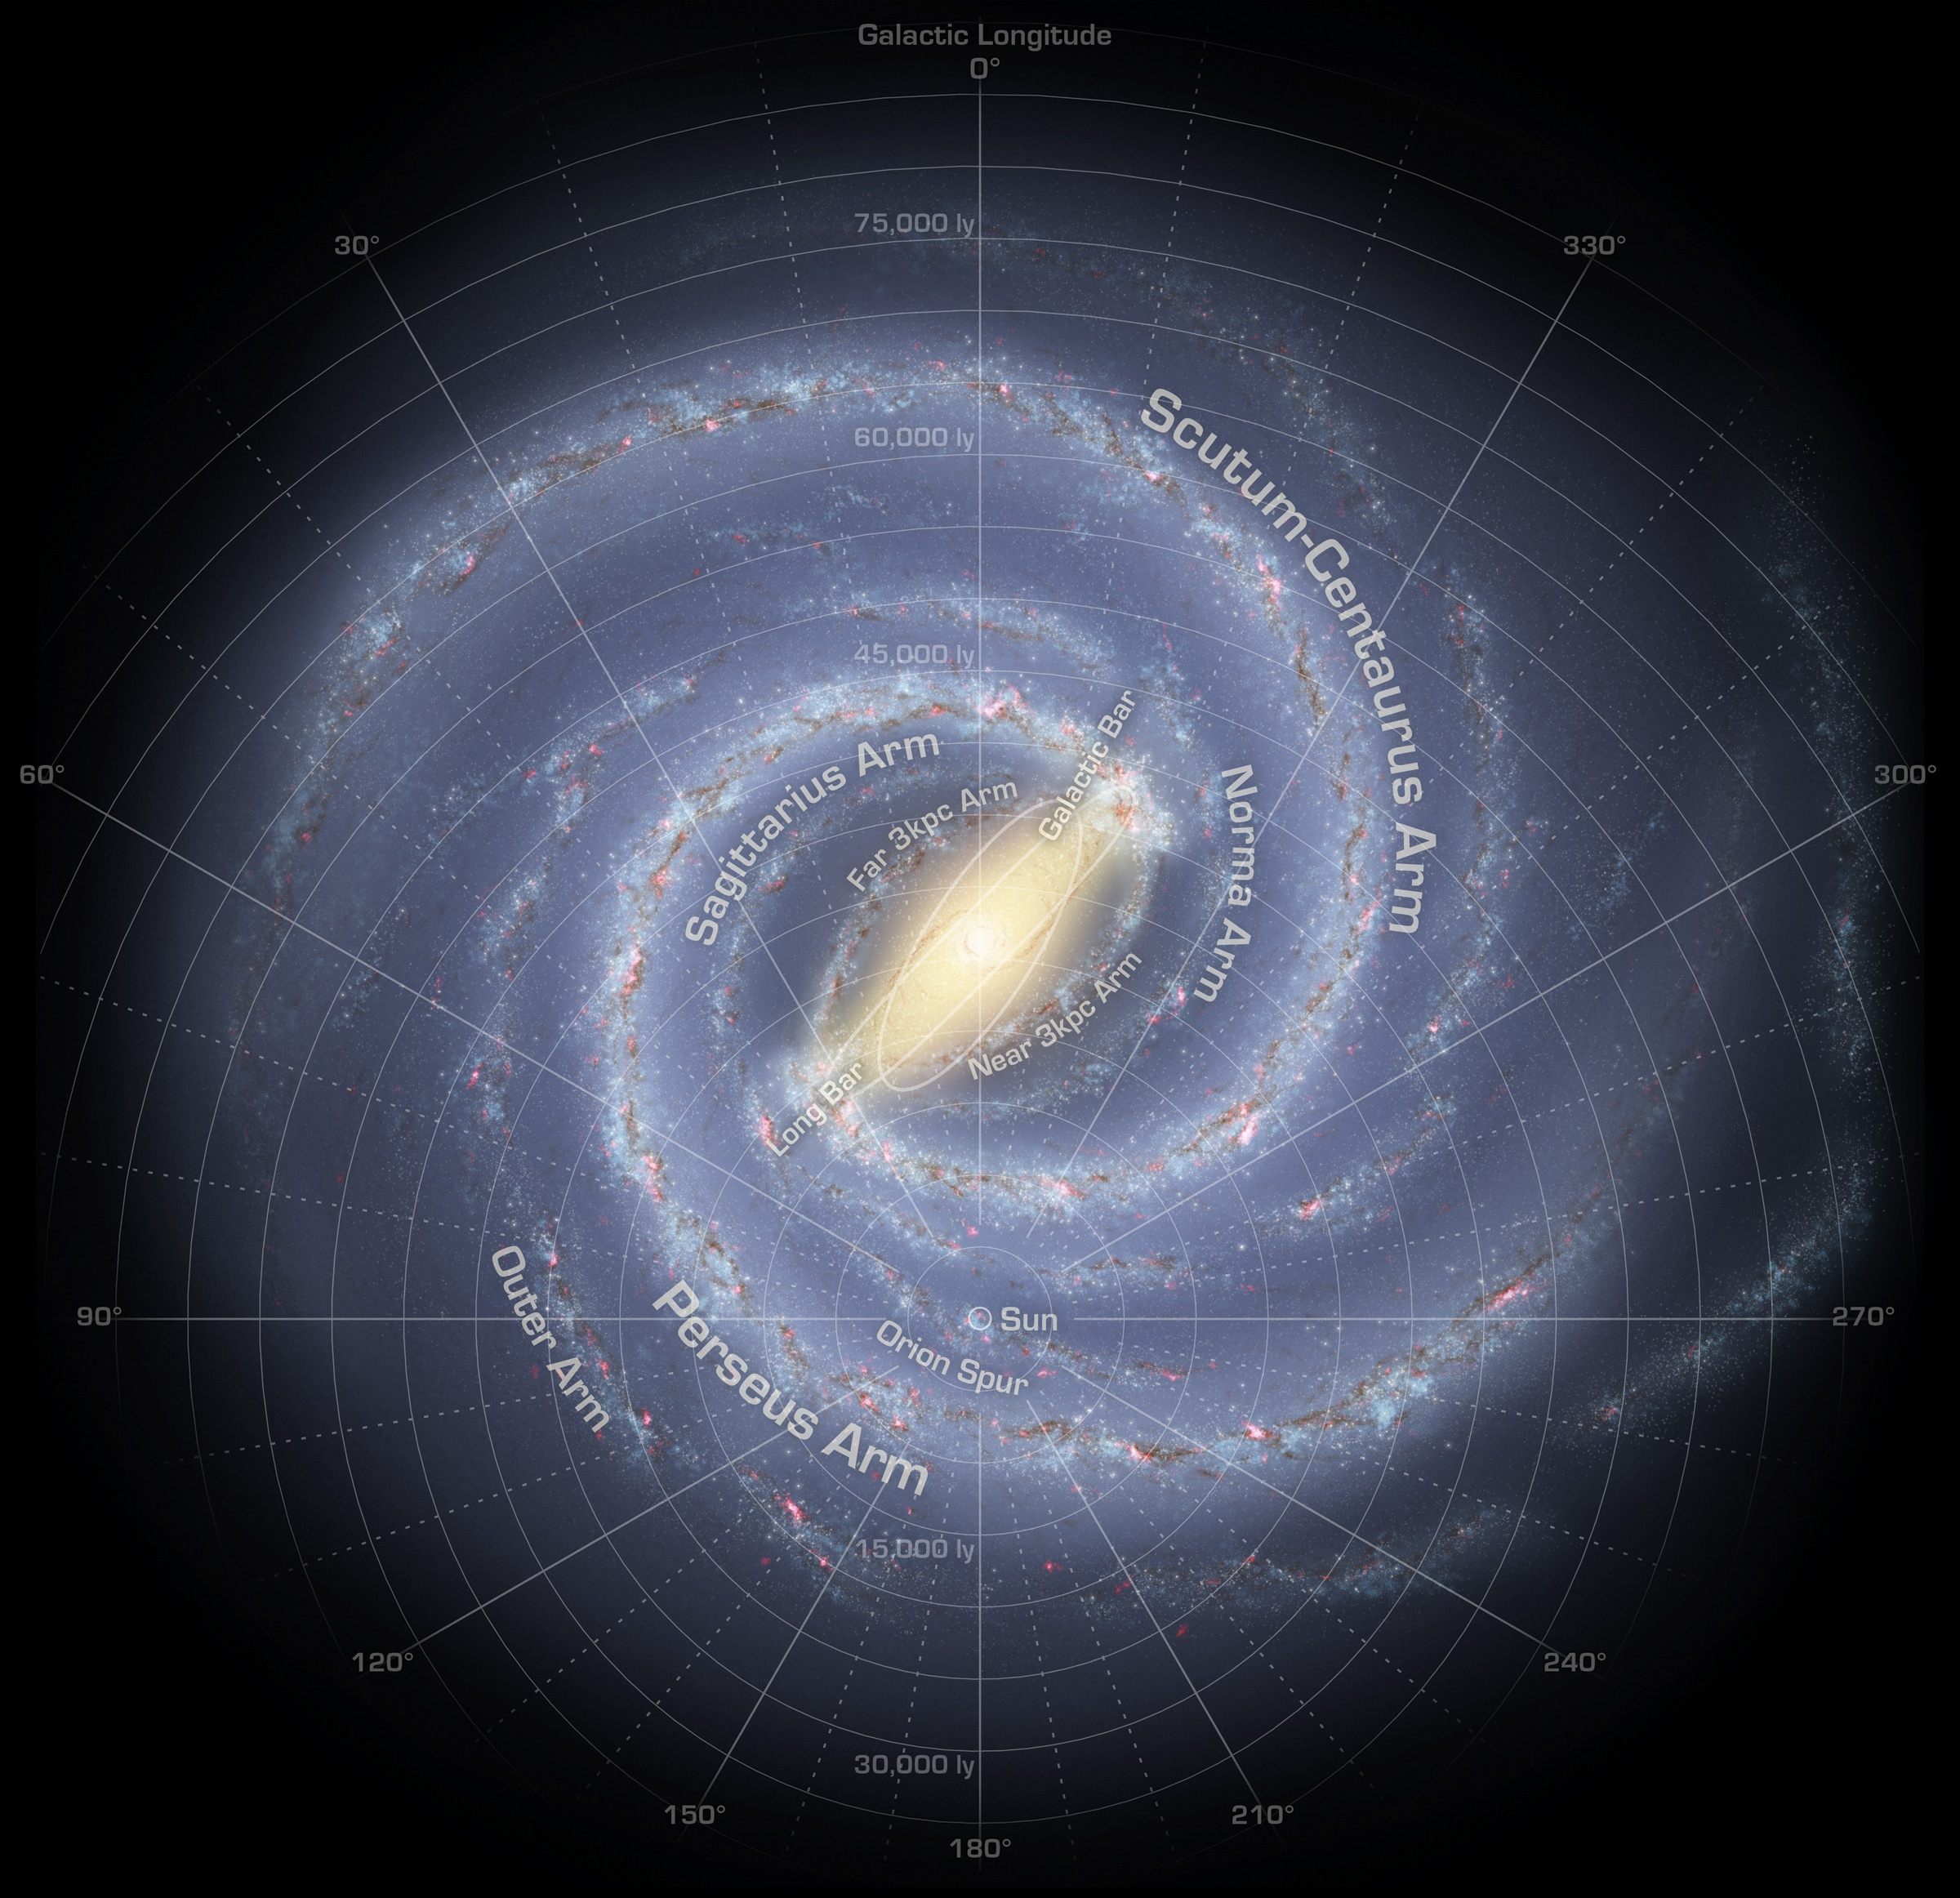
\includegraphics[width=\textwidth]{images/milkyway_structure_big_crop.jpeg}
    \end{column}%
    \begin{column}{0.5\textwidth}%
      \only<1>{%
      \begin{tikzpicture}[overlay, remember picture, shift={(current page.center)}]%
        \draw[red!70!black, thick, o->] (-3.895, -1.52) -- +(55:5);%
      \end{tikzpicture}%
      \begin{tikzpicture}%
        \begin{axis}[%
            title={$T_b$ für $l=\SI{335}{\degree}$},
            xmin=21.09,
            xmax=21.12,
            ymin=-10,
            ymax=120,
            width=\textwidth,
            xlabel={\SIQ{λ}{\centi\meter}},
            ylabel={$\SIQ{T_b}{\kelvin}$},
          ]%
          \addplot[red!70!black] table[x index=3, y index=1]{./data/radial_velocity_l335.txt};%
        \end{axis}%
      \end{tikzpicture}%
      }%
      \only<2>{%
      \begin{tikzpicture}[overlay, remember picture, shift={(current page.center)}]%
        \draw[red!70!black, thick, o->] (-3.935, -1.44) -- +(0:4);
      \end{tikzpicture}%
      \begin{tikzpicture}%
        \begin{axis}[
            title={$T_b$ für $l=\SI{270}{\degree}$},
            xmin=21.09,
            xmax=21.12,
            ymin=-10,
            ymax=120,
            width=\textwidth,
            xlabel={\SIQ{λ}{\centi\meter}},
            ylabel={$\SIQ{T_b}{\kelvin} $},
          ]%
          \addplot[red!70!black] table[x index=3, y index=1]{./data/radial_velocity_l270.txt};%
        \end{axis}%
      \end{tikzpicture}%
      }%
    \end{column}%
  \end{columns}%
\end{frame}

\fullscreenimage{./images/things.png}
\end{document}
